%***Getting the right predictions for SoC, SoH, and RUL is \textbf{ML} algorithms that learn from examples, such as SVMs and Random Forests, have been used to predict SoC and SoH using features like voltage, current, and temperature. For example, \cite{sun_simultaneous_2022} shows SVMs getting high accuracy in SoH estimation (98.26\%) for lead-acid batteries under controlled conditions. However, these methods need a lot of feature engineering and have trouble with time-based patterns. On the contrary, \textbf{Deep Learning} models are very good at finding time-based and spatial patterns in battery data. K...ery important for making batteries work better in cars and trains. These predictions help make BMS more reliable and work better. They provide key information for watching battery health and planning when to fix or replace batteries. Traditional methods, like Coulomb Counting and Kalman Filters, often have trouble with complex battery behavior and changing conditions. New advances in AI, especially ML and deep learning, provide better solutions by finding complex patterns in battery data. This chapter looks at the current best methods for SoC, SoH, and RUL estimation, fo...********************************************
\chapter{State of the Art}
\label{ch:stateoftheart}
%************************************************
Getting the right predictions for SoC, SoH, and RUL is very important for making batteries work better in cars and trains. These predictions help make battery management systems (BMS) more reliable and work better. They provide key information for watching battery health and planning when to fix or replace batteries. Traditional methods, like Coulomb Counting and Kalman Filters, often have trouble with complex battery behavior and changing conditions. New advances in AI, especially machine learning and deep learning, provide better solutions by finding complex patterns in battery data. This chapter looks at the current best methods for SoC, SoH, and RUL estimation, focusing on AI-based approaches.

\section{Battery State Estimation}

\subsection{Traditional Methods}
\label{subsec:traditional_methods}
Traditional methods for checking battery state can be put into two groups: physics-based and statistical approaches, each with built-in problems.

\textbf{Physics-Based Methods} create models of how batteries work chemically and electrically. Key approaches include:
\begin{itemize}
    \item \textbf{Equivalent Circuit Models (ECMs)}: Show batteries using electrical parts (like resistors, capacitors) to copy voltage and current behavior. ECMs represent battery dynamics through simplified electrical circuits that capture the essential electrochemical behaviors while maintaining computational efficiency. Figure~\ref{fig:ecm_models} illustrates two common ECM configurations: (a) the Thévenin model with a single RC pair representing charge transfer resistance and double-layer capacitance, and (b) the PNGV model with multiple RC pairs capturing different time constants in battery response. These models include internal resistance ($R_0$), polarization resistances ($R_{Th}$, $R_{pa}$, $R_{pc}$), and corresponding capacitances ($C_{Th}$, $C_{pa}$, $C_{pc}$) to model various electrochemical processes. ECMs are fast to compute and suitable for real-time applications, but they are not very accurate when conditions change and require parameter identification for different operating conditions \cite{tran_comparative_2021}.
    \label{subsec:ecm_models}

\begin{figure}[htbp]
\centering
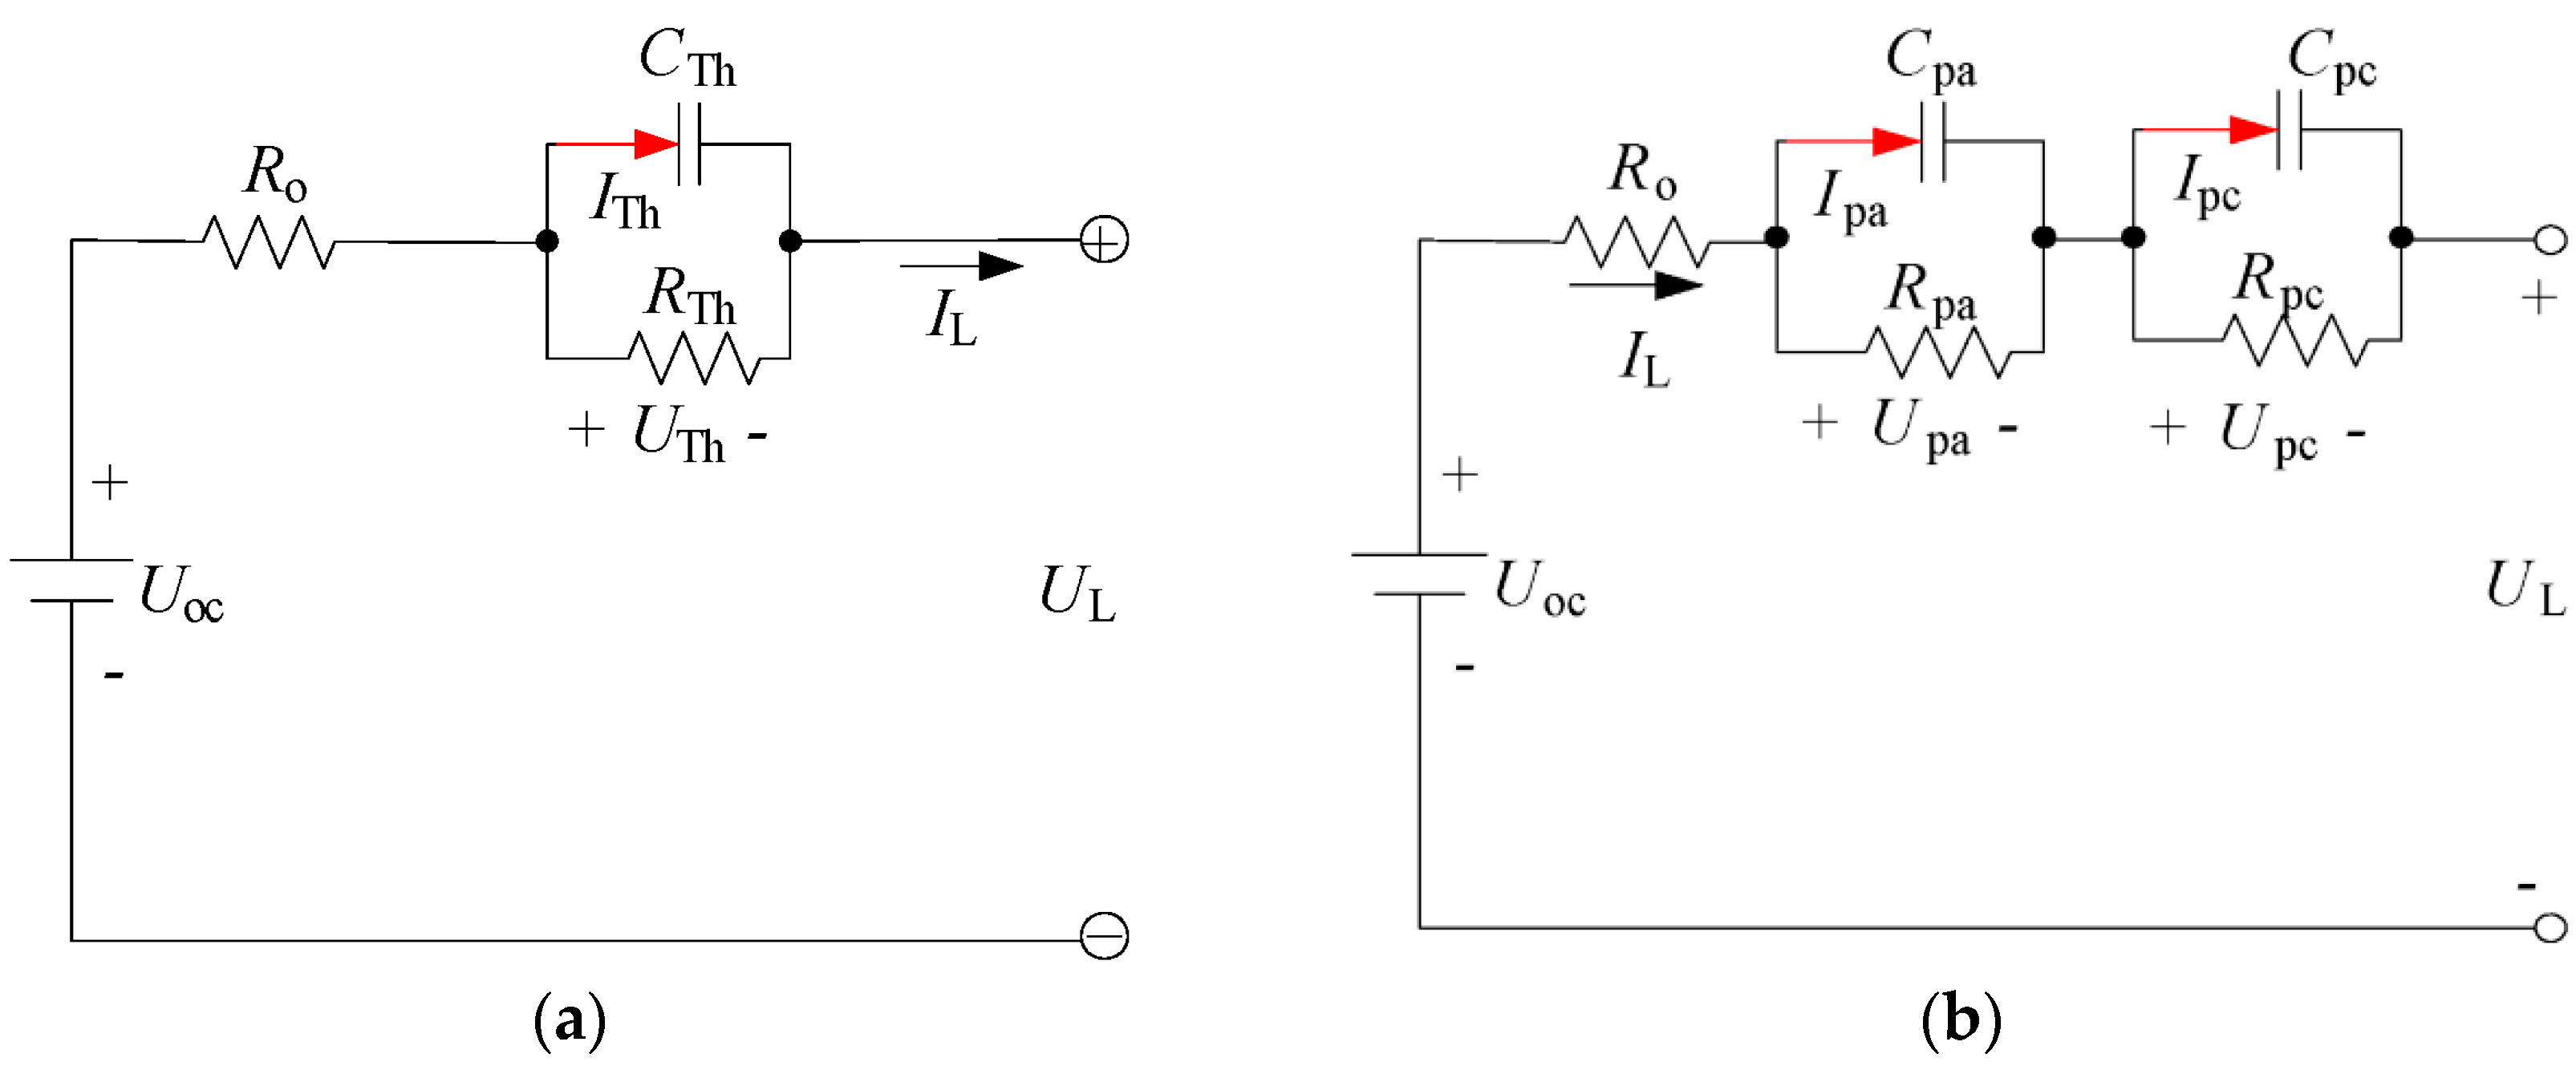
\includegraphics[width=1.0\textwidth]{imgs/ECM_1st_2nd_order.png}
\caption{Equivalent Circuit Models (ECMs) showing (a) Thévenin model with single RC pair and (b) PNGV model with multiple RC pairs. These models use electrical components to represent battery electrochemical behavior, where $R_0$ represents ohmic resistance, $R_{Th}/C_{Th}$ and $R_{pa}/C_{pa}$, $R_{pc}/C_{pc}$ represent different polarization effects with their respective time constants \cite{tran_comparative_2021}.}
\label{fig:ecm_models}
\end{figure}

    \item \textbf{Electrochemical Models}: Copy internal chemical reactions, giving high accuracy but needing a lot of computer power and detailed knowledge of battery parameters. These models are based on fundamental electrochemical principles and describe the physical and chemical processes occurring within battery cells, including ion transport, charge transfer reactions, and material phase changes \cite{mama_comprehensive_2025}. Electrochemical models typically solve complex partial differential equations that describe mass and charge conservation, making them computationally intensive but highly accurate for predicting battery behavior under various operating conditions.

    A notable example of modern electrochemical modeling frameworks is BattMo (Battery Modeling in MATLAB), an open-source battery simulation platform that provides comprehensive tools for electrochemical battery modeling \cite{noauthor_battmo_2024}. BattMo offers advanced capabilities including multi-physics coupling, detailed electrode modeling, and thermal effects integration, making it suitable for research and development applications.

    During the initial phases of this research, BattMo was evaluated as a potential modeling framework for generating synthetic battery data and understanding fundamental battery behavior. The platform's comprehensive approach to electrochemical modeling and its integration with MATLAB made it an attractive option for physics-based battery simulation. However, after preliminary exploration, the focus shifted toward data-driven approaches due to the computational complexity requirements and the need for extensive parameter identification that electrochemical models demand for practical applications in real-time battery management systems.
\end{itemize}

Unlike these, \textbf{ statistical methods} use real data to estimate battery states. Common methods include:
\begin{itemize}
    \item \textbf{Coulomb Counting}: This method estimates SoC by integrating current over time, following the fundamental principle that charge accumulation equals the integral of current. While conceptually straightforward, coulomb counting suffers from significant practical limitations including sensitivity to measurement noise, current sensor drift, and initialization errors. Figure~\ref{fig:current_integration_error} illustrates how current integration errors accumulate over time, demonstrating the inherent challenges of this approach. The method's accuracy degrades particularly under varying sampling rates and temperature conditions~\cite{noauthor_implementation_nodate}. Despite these limitations, coulomb counting remains widely used due to its computational simplicity, often serving as a baseline method or being combined with other estimation techniques for improved reliability~\cite{movassagh_critical_2021}.

\begin{figure}[htbp]
\centering
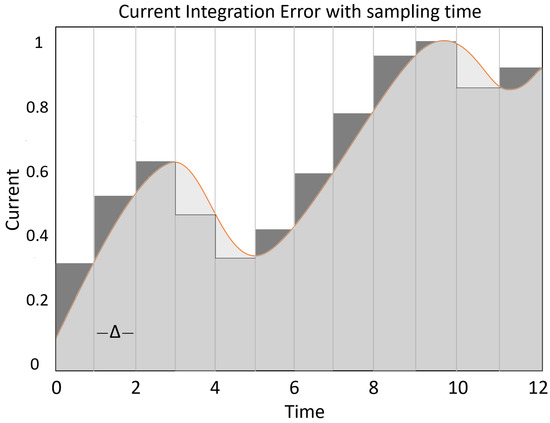
\includegraphics[width=0.8\textwidth]{imgs/coulomb.jpg}
\caption{Current integration error accumulation over time showing how measurement uncertainties and sampling effects impact coulomb counting accuracy. The step-like behavior demonstrates the discrete nature of current sampling, while the smooth curve represents the theoretical continuous integration~\cite{movassagh_critical_2021}.}
\label{fig:current_integration_error}
\end{figure}

    \item \textbf{Kalman Filters}: Kalman filters represent a sophisticated recursive approach to state estimation that optimally combines model predictions with noisy measurements using statistical principles. The filter operates in two phases: prediction (using system dynamics) and correction (incorporating new measurements). For battery applications, the EKF is commonly employed to handle the nonlinear relationship between battery states and observable quantities such as terminal voltage~\cite{mastali_battery_2013}. Figure~\ref{fig:ekf_diagram} illustrates the EKF estimation process, showing how the algorithm iteratively refines state estimates by balancing model predictions with measurement data. While Kalman filters provide optimal estimates under Gaussian noise assumptions, their performance degrades significantly when dealing with the complex nonlinear dynamics and time-varying parameters characteristic of battery systems. The method requires accurate system models and proper tuning of noise covariance matrices, which can be challenging in practical applications where battery parameters drift over time due to aging and temperature variations~\cite{becker_wwwkalmanfilternet_online_nodate}.

\begin{figure}[htbp]
\centering
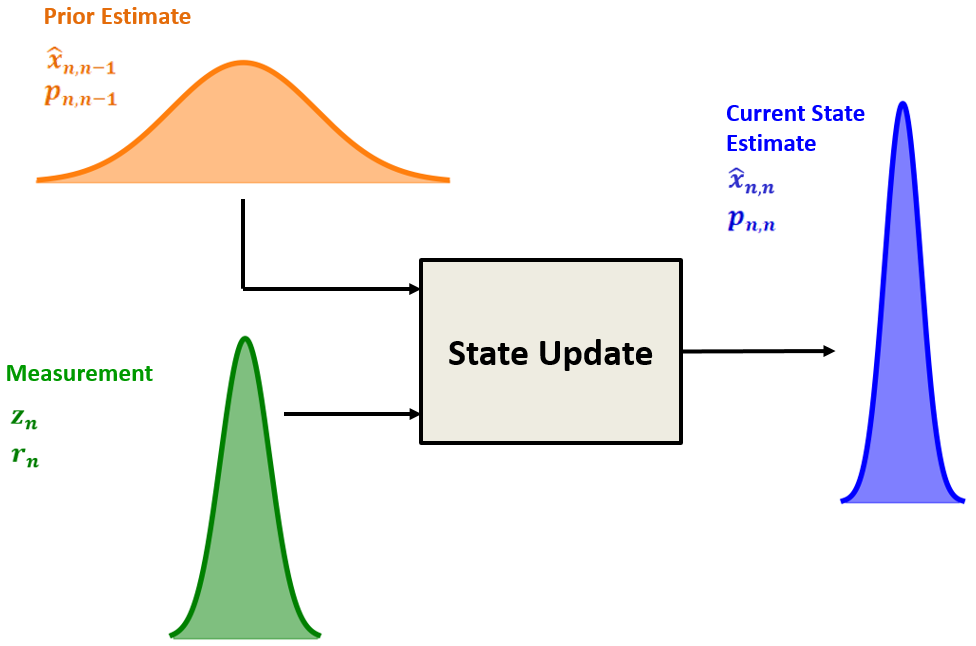
\includegraphics[width=0.9\textwidth]{imgs/ekf.png}
\caption{EKF State estimation process showing Prior Estimate (orange), Measurement (green), State Update (gray), and Current State Estimate (blue).~\cite{becker_wwwkalmanfilternet_online_nodate}.}
\label{fig:ekf_diagram}
\end{figure}
    
\end{itemize}

Because these methods often fail to capture small changes in battery behavior when conditions change, multiple AI-based approaches have been proposed in the last decade.

\subsection{AI-Based Methods}
\label{subsec:ai_methods}
AI-based methods use machine learning and deep learning to model complex relationships in battery data. This section looks at key approaches, datasets, and how they're used in this project.

\textbf{Machine Learning} algorithms that learn from examples, such as Support Vector Machines (SVMs) and Random Forests, have been used to predict SoC and SoH using features like voltage, current, and temperature. For example, \cite{sun_simultaneous_2022} shows SVMs getting high accuracy in SoH estimation (98.26\%) for lead-acid batteries under controlled conditions. However, these methods need a lot of feature engineering and have trouble with time-based patterns. On the contrary, \textbf{Deep Learning} models are very good at finding time-based and spatial patterns in battery data. Key types include:
\begin{itemize}
    \item \textbf{CNNs}: Find spatial features from battery data, such as voltage profiles. Combining CNNs with LSTM units, as done in the \cite{Fangfang_Yang} paper, makes forecasting more accurate by modeling time-based patterns.
    \item \textbf{RNNs and LSTMs}: Made for sequential data, LSTMs are very good for RUL prediction, as they capture long-term battery wear trends. The key advantage of LSTMs over traditional RNNs lies in their ability to selectively remember and forget information through specialized gate mechanisms, as illustrated in Figure~\ref{fig:rnn_vs_lstm_comparison}. While standard RNNs suffer from vanishing gradient problems that limit their ability to capture long-term dependencies, LSTMs incorporate long-term memory cells alongside working memory, enabling effective modeling of extended battery degradation sequences. This architectural improvement is crucial for battery applications where degradation patterns span hundreds or thousands of cycles \cite{noauthor_phenomnet_nodate}. Studies using the NASA Battery Dataset \cite{noauthor_nasa_nodate} show LSTM-based models work better than older methods in RUL estimation as done in the \cite{hong_state--health_2023}.

\begin{figure}[htbp]
\centering
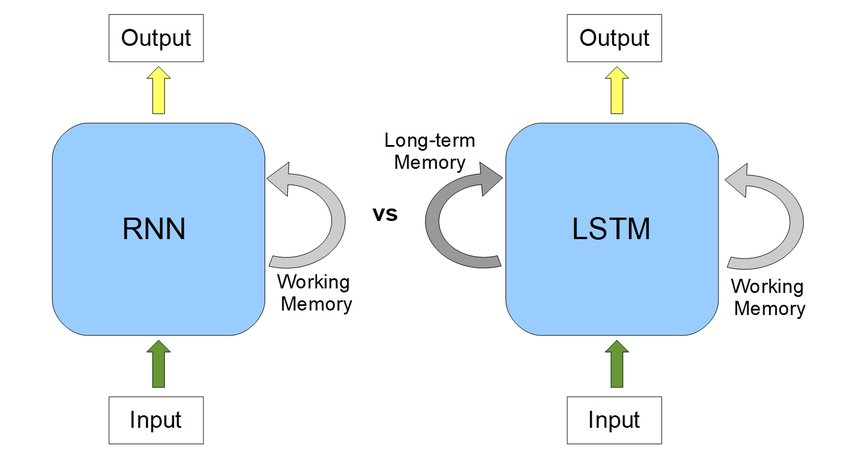
\includegraphics[width=1\textwidth]{imgs/rnn_lstm.png}
\caption{Comparison between RNN and LSTM architectures showing the fundamental difference in memory mechanisms. RNNs rely solely on working memory with limited long-term retention capabilities, while LSTMs incorporate both working memory and long-term memory cells, enabling better modeling of extended temporal dependencies in battery degradation data \cite{noauthor_phenomnet_nodate}.}
\label{fig:rnn_vs_lstm_comparison}
\end{figure}

    \item \textbf{Transformer Models}: New in battery state estimation, transformers use attention mechanisms to model complex dependencies, showing promise in handling different-length sequences \cite{yilmaz_transformer-based_2025}. The Transformer architecture, illustrated in Figure~\ref{fig:transformer_detailed_architecture}, consists of an encoder-decoder structure with multiple specialized components. The encoder processes input sequences through multiple layers containing self-attention mechanisms, positional encoding, and feed-forward networks, enabling the model to capture long-range dependencies in battery time series data. The decoder utilizes both self-attention and encoder-decoder attention mechanisms to generate predictions, with linear mapping layers producing the final output. This architecture is particularly effective for battery applications because the attention mechanisms can automatically identify relevant temporal patterns and relationships between different time steps in battery degradation sequences, eliminating the need for manual feature engineering while maintaining computational efficiency through parallel processing capabilities.
\end{itemize}

\begin{figure}[htbp]
\centering
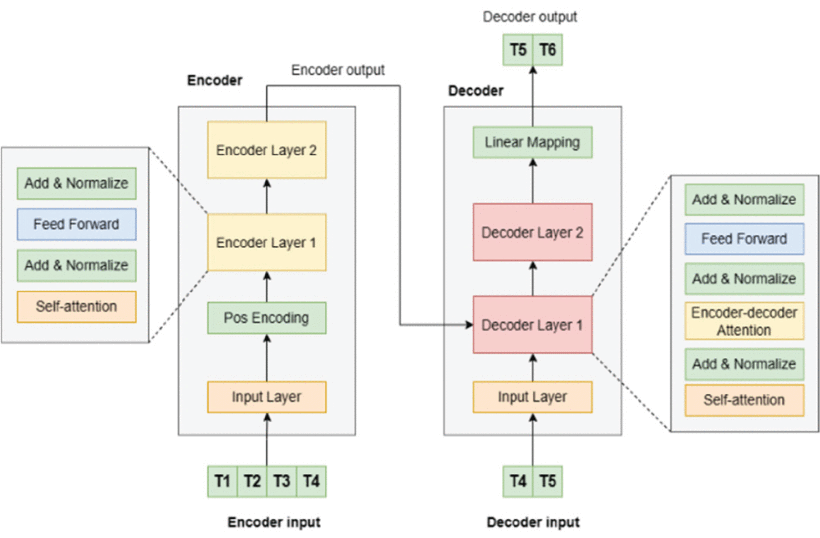
\includegraphics[width=0.9\textwidth]{imgs/transformer_input.png}
\caption{Detailed Transformer architecture showing the encoder-decoder structure with self-attention mechanisms, positional encoding, and feed-forward networks. The encoder processes input sequences (T1-T4) while the decoder generates output predictions (T5-T6) using attention mechanisms to capture temporal dependencies in battery data.}
\label{fig:transformer_detailed_architecture}
\end{figure}

\subsection{Hybrid Approaches}
Hybrid models combine physics-based and data-driven methods to make results more accurate. For example, some studies combine ECMs talked earlier, with neural networks to improve SoC estimates, using physical constraints to reduce the amount of training data needed \cite{dini_exploiting_2025}. Such approaches are very useful for railway applications, where operating conditions change a lot. Despite improvements, several challenges still exist in battery state estimation. \textbf{Data requirements} pose a significant challenge as NN models, especially deep learning, need large, varied datasets. \textbf{Computational complexity} presents another obstacle since real-time estimation in cars and trains needs fast models, which is a challenge for complex deep learning systems. Finally, the \textbf{lack of standard datasets} remains problematic as the absence of universal, open-source datasets for our applications limits model comparison and testing.


\section{Datasets for AI-Based Estimation}
\label{subsec:datasets}
The quality and variety of datasets are very important for training strong AI models. A comprehensive analysis of available battery datasets reveals significant variation in data completeness, experimental conditions, and feature availability. Table~\ref{tab:battery_datasets_comparison} presents a detailed comparison of notable publicly available battery datasets, highlighting their characteristics and available measurements.

\begin{table}[htbp]
\centering
\caption{Comprehensive comparison of available battery datasets and their features}
\label{tab:battery_datasets_comparison}
\resizebox{\textwidth}{!}{%
\begin{tabular}{lcccccccccccccccc}
\hline
\textbf{Dataset} & \textbf{Cell Type} & \textbf{Chemistry} & \textbf{Time} & \textbf{C/D Ind.} & \textbf{Cycle} & \textbf{Current} & \textbf{Voltage} & \textbf{Dis. Cap.} & \textbf{Ch. Cap.} & \textbf{Ch. Energy} & \textbf{Dis. Energy} & \textbf{dV/dt} & \textbf{Int. Res.} & \textbf{AC Imp.} & \textbf{ACI Phase} & \textbf{Temp.} \\
\hline
Zn-ion, Na-ion @2025 & Various & Zn-ion, Na-ion & $\checkmark$ & $\checkmark$ & & $\checkmark$ & $\checkmark$ & $\checkmark$ & $\checkmark$ & & & & & & & \\
CALCE CS2 @2010 & Prismatic & LiCoO2 & $\checkmark$ & $\checkmark$ & $\checkmark$ & $\checkmark$ & $\checkmark$ & $\checkmark$ & $\checkmark$ & $\checkmark$ & $\checkmark$ & $\checkmark$ & $\checkmark$ & $\pm$ & $\pm$ & Initial \\
MATR @2019 & 18650 & LFP/graphite & $\checkmark$ & $\checkmark$ & $\checkmark$ & $\checkmark$ & $\checkmark$ & $\checkmark$ & $\checkmark$ & $\checkmark$ & $\checkmark$ & $\checkmark$ & $\checkmark$ & & & $\checkmark$ \\
MATR @2019 CL & 18650 & LFP/graphite & $\checkmark$ & & $\checkmark$ & $\checkmark$ & $\checkmark$ & $\checkmark$ & $\checkmark$ & $\checkmark$ & $\checkmark$ & $\checkmark$ & & & & $\checkmark$ \\
HUST @2022 & Various & LFP/graphite & $\checkmark$ & $\pm$ & $\checkmark$ & $\checkmark$ & $\checkmark$ & $\checkmark$ & $\checkmark$ & & & & & & & \\
RWTH @2017 & 18650 & Lithium Ion & $\checkmark$ & $\checkmark$ & $\checkmark$ & $\checkmark$ & $\checkmark$ & $\checkmark$ & $\checkmark$ & $\checkmark$ & $\checkmark$ & & & & & $\checkmark$ \\
ISU-ILCC @2023 & 502030 & Li-polymer & $\checkmark$ & & & $\checkmark$ & $\checkmark$ & $\checkmark$ & $\checkmark$ & $\checkmark$ & $\checkmark$ & & & & & \\
XJTU @2022 & 18650 & NCM Li-ion & $\checkmark$ & & & $\checkmark$ & $\checkmark$ & $\checkmark$ & $\checkmark$ & & & & & & & $\checkmark$ \\
Tongji @2022 & 18650 & NCA/NCM & $\checkmark$ & & $\checkmark$ & $\checkmark$ & $\checkmark$ & $\checkmark$ & $\checkmark$ & & & & & & & \\
Stanford @2024 & 21700 & Graphite/Si & $\checkmark$ & & $\checkmark$ & $\checkmark$ & $\checkmark$ & $\checkmark$ & $\checkmark$ & $\checkmark$ & $\checkmark$ & $\checkmark$ & $\checkmark$ & & & $\checkmark$ \\
\hline
\end{tabular}}
\end{table}

The analysis reveals several key insights about the current state of battery datasets:

Notable datasets with comprehensive feature sets include:
\begin{itemize}
    \item \textbf{NASA Battery Dataset} \cite{noauthor_nasa_nodate}: Provides voltage, current, temperature, and impedance data under different operating conditions, widely used for SoC and RUL estimation due to its diverse experimental scenarios and comprehensive measurement suite.
    \item \textbf{CALCE Battery Dataset} \cite{CALCE_battery_nodate}: Contains extensive aging data from lithium-ion batteries under different stress conditions, particularly valuable for SoH estimation and understanding battery degradation patterns. Notable for its complete feature set including energy measurements and impedance data.
    \item \textbf{MATR Battery Dataset} \cite{MATR_dataset_nodate}: Provides high-quality data from automotive battery testing, focusing on real-world driving conditions and temperature variations with comprehensive measurement capabilities.
    \item \textbf{Stanford Dataset}: Offers the most recent data with advanced battery chemistries (graphite/silicon) and comprehensive measurements including internal resistance and energy metrics.
\end{itemize}
These datasets show the importance of including real-world operating conditions and diagnostic measurements to make models work better in different situations.

%The \textit{BattAIHealth} project addresses these gaps by developing AI models trained on both synthetic and real-world datasets, making them work better and be suitable for real-time use in transportation systems.

\section{Discussion}
The current best methods in battery state estimation show a move from older physics-based and statistical methods to AI-driven approaches. While machine learning and deep learning models, supported by datasets like the NASA Battery Dataset and Aging Dataset from EV, give better accuracy, challenges such as limited data and changing operating conditions still exist. This project builds on these improvements by developing strong AI models made for car and train applications, aiming to make BMS more reliable and work better.